\begin{document}

%----------------------------------------------------------------- %
{Correlation}
\vspace{-0.5cm}
\begin{figure}
\centering
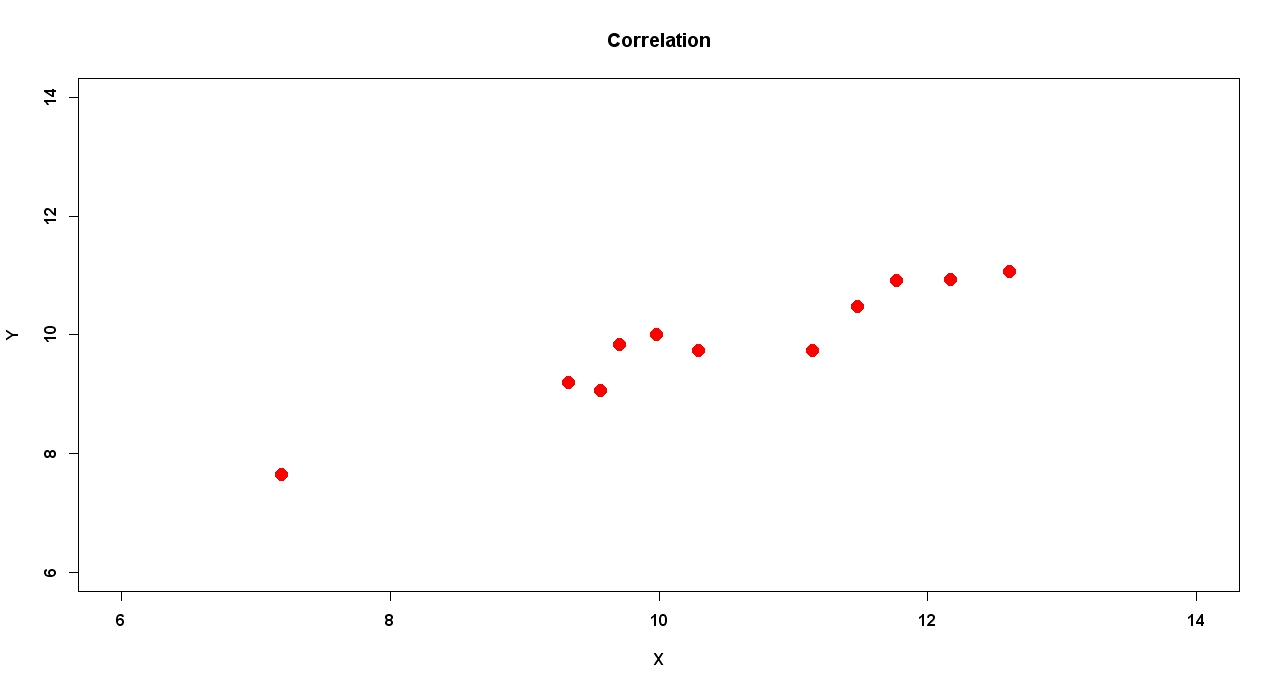
\includegraphics[width=1.05\linewidth]{../IntroStats/CorTest1}
\section{Correlation test}

Assessment of tuna quality: We compare the Hunter L measure of
lightness to the averages of consumer panel scores (recoded as
integer values from 1 to 6 and averaged over 80 such values) in
9 lots of canned tuna.
(Hollander \& Wolfe (1973), p. 187f.)

\begin{verbatim}
x <- c(44.4, 45.9, 41.9, 53.3, 44.7, 44.1, 50.7, 45.2, 60.1)
y <- c( 2.6,  3.1,  2.5,  5.0,  3.6,  4.0,  5.2,  2.8,  3.8)
\end{verbatim}

\begin{itemize}

\item Test the hypothesis that the correlation coefficient is not zero.
\item Test the hypothesis that the correlation coefficient is positive.
\item What is the test statistics in both cases?
\item What is the p-value in both cases?
\item Interpret the p-values.
\end{itemize}


The alternative hypothesis of interest is there is a correlation between the
Hunter L value and the panel score.

\begin{verbatim}
> cor.test(x, y , alternative = "two.sided")

Pearson's product-moment correlation

data:  x and y
t = 1.8411, df = 7, p-value = 0.1082
alternative hypothesis: true correlation is not equal to 0
95 percent confidence interval:
-0.1497426  0.8955795
sample estimates:
cor
0.5711816

\end{verbatim}


The alternative hypothesis of interest is that the
Hunter L value is positively associated with the panel score.
\begin{verbatim}
> cor.test(x, y, alternative = "greater")

Pearson's product-moment correlation

data:  x and y
t = 1.8411, df = 7, p-value = 0.05409
alternative hypothesis: true correlation is greater than 0
95 percent confidence interval:
-0.02223023  1.00000000
sample estimates:
cor
0.5711816
\end{verbatim}

\begin{verbatim}
> ct2 <- cor.test(x, y, alternative = "greater")
> names(ct2)
[1] "statistic"   "parameter"   "p.value"   "estimate"  "null.value"  "alternative" "method"      "data.name"
[9] "conf.int"
>
> ct2$p.value
[1] 0.05408653
>
> ct2$statistic
t
1.841083
\end{verbatim}




\end{figure}
{
\Large
Correlation Coefficient : $r = 0.922$
}

%----------------------------------------------------------------- %
{Correlation}
\vspace{-0.5cm}
\begin{figure}
\centering
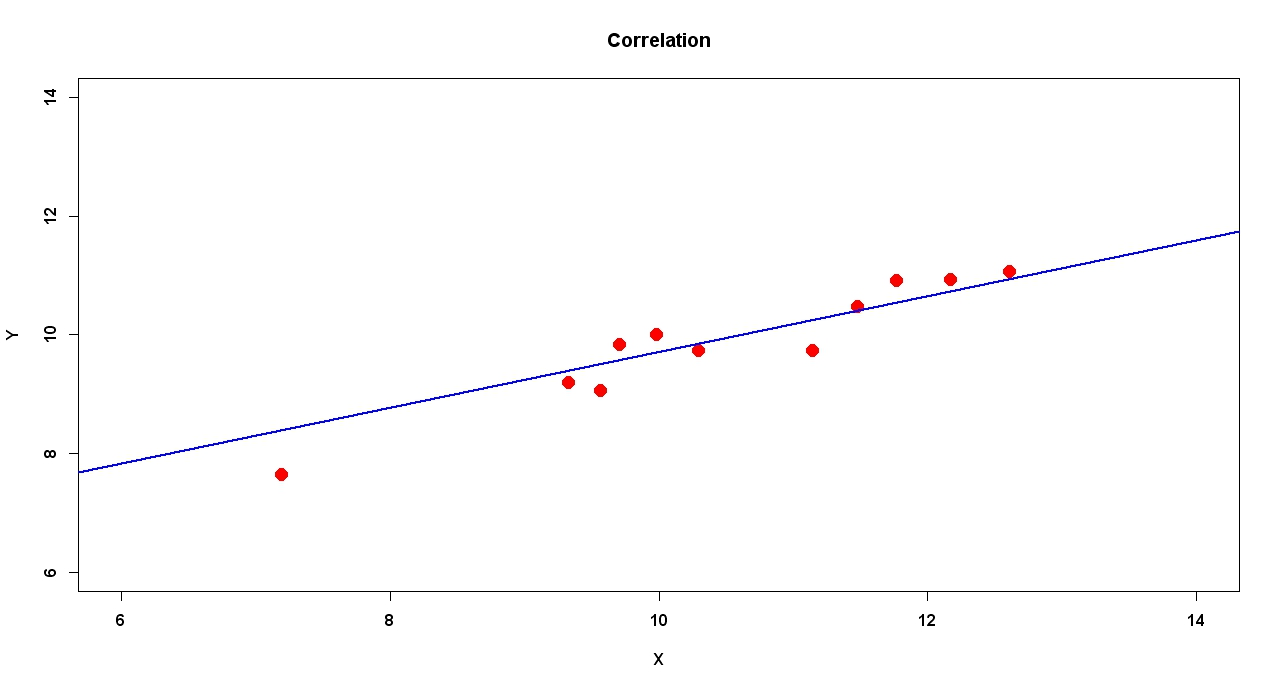
\includegraphics[width=1.05\linewidth]{../IntroStats/CorTest2}
\end{figure}
{
\Large
Correlation Coefficient : $r = 0.922$
}

%----------------------------------------------------------------- %
{Correlation}
\begin{figure}
\centering
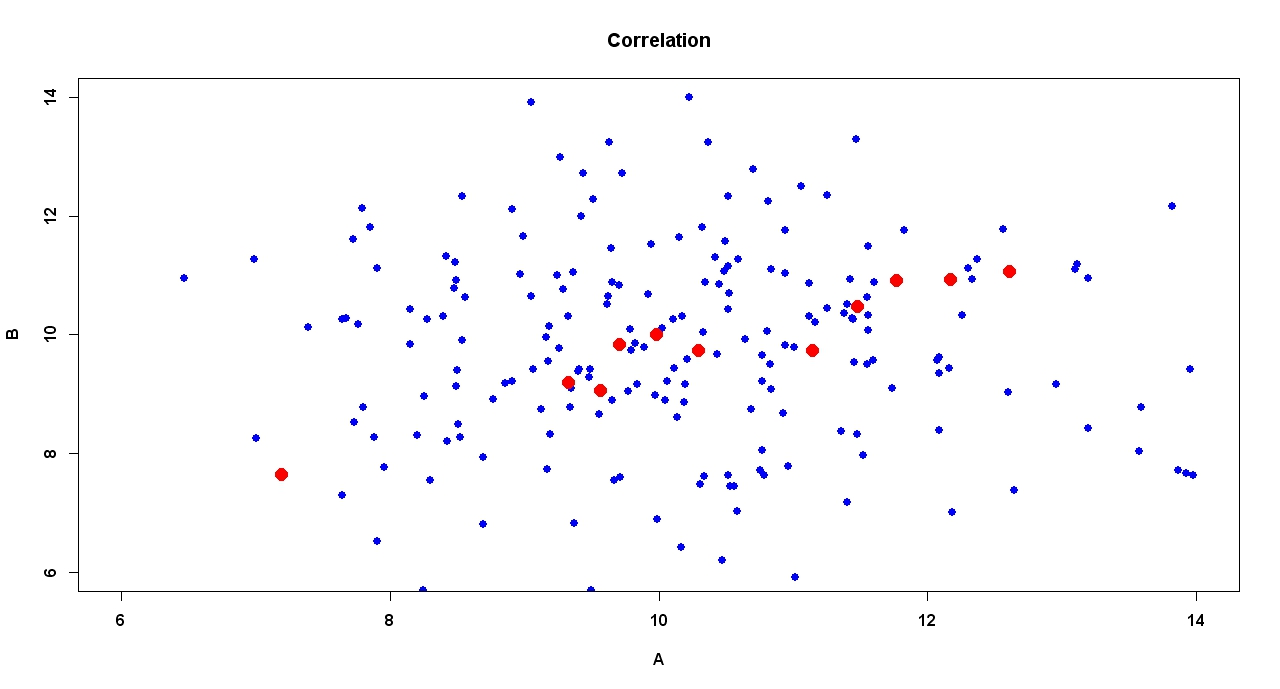
\includegraphics[width=1.05\linewidth]{../IntroStats/CorTest3}
\end{figure}
{
\Large
True Correlation Coefficient : $rho \approx 0$
}



%CORRELATION
\subsection{Correlation and cause-effect}
\begin{itemize}
\item Note that a strong relationship between two variables does not
imply a cause-effect relationship.
\item For example, there is a strong negative correlation between the
sales of ice cream and the number of flu infections.
\item This does not mean that ice cream protects against flu.
\item This relationship results from a latent variable (a variable that has
not been observed).
\item Such a latent variable in this case is the weather. Low
temperatures and wet weather result in a high number of flu
infections and low ice cream sales. \item Hot, sunny weather leads to the
opposite.
\end{itemize}



%---------------------------------------------------------------------%

\subsection{Properties of the Correlation Coefficient}
Example: We are given data for 6 graduates. Below is their
final QCA and their corresponding starting salary after
graduation.

% Subject 1 2 3 4 5 6
% Final QCA 2.8 3.4 3.2 3.8 3.2 3.4
% Starting Salary 20 000 24 500 23 000 25 000 20 000 22 500

Calculate the sample correlation coefficient.


%--------------------------------------------------------------------%
\section{Calculating Correlation from Sums of Squares}
\subsection{Identities}
\begin{itemize}
\item $S_{XY} = -283.8$
\item $S_{XX} = 613.6$
\item $S_{YY} = 148.9$
\item $\sum(X_i)  = 318 $
\item $\sum(Y_i)  = 61$
\end{itemize}

\begin{itemize}
\item Calculate the correlation coefficient and interpret its value.
\item The correlation coefficient is computed using the following formula:
\[ r_{X,Y} = \frac{\S_{XY}}{\sqrt{\S_{XX}\S_{YY}}} \]
\item From the values given
\[ r_{X,Y} = \frac{-283.8}{\sqrt{(613.6)(148.9)}} = -0.9389 \]
\item Very strong negative linear relationship
\end{itemize}



\begin{figure}
\centering
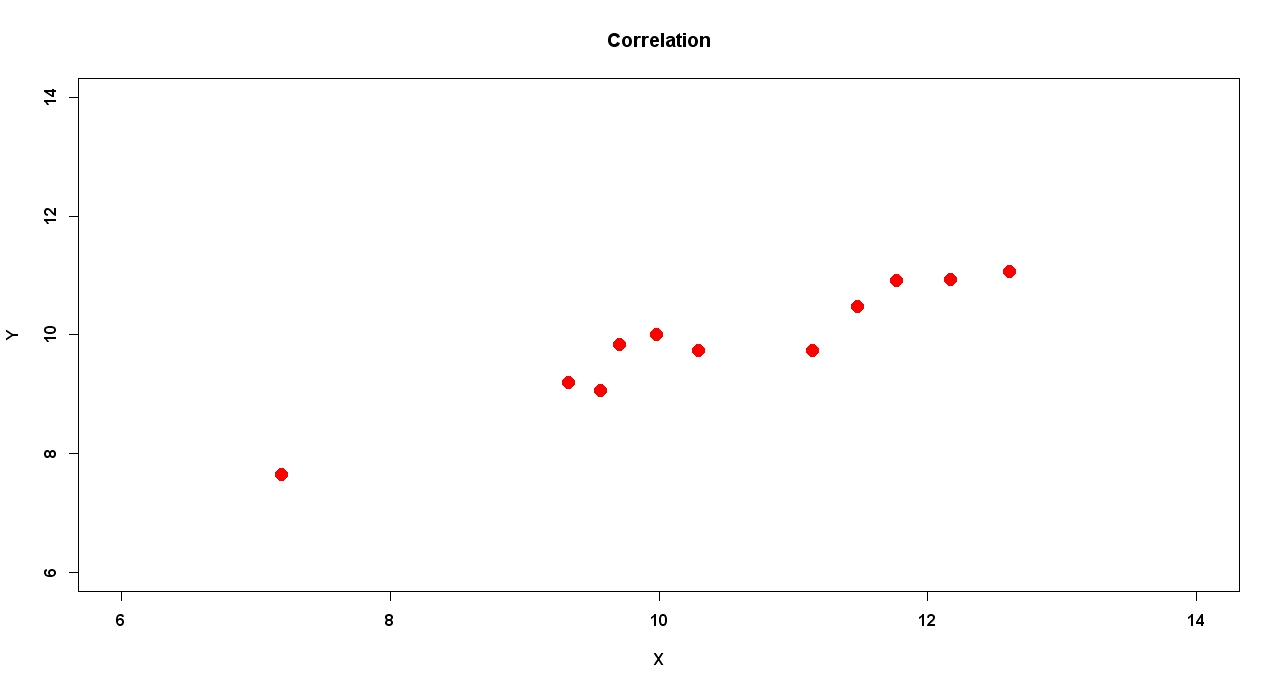
\includegraphics[width=1.05\linewidth]{../IntroStats/CorTest1}
\end{figure}
{

Correlation Coefficient : $r = 0.922$
}



\begin{figure}
\centering
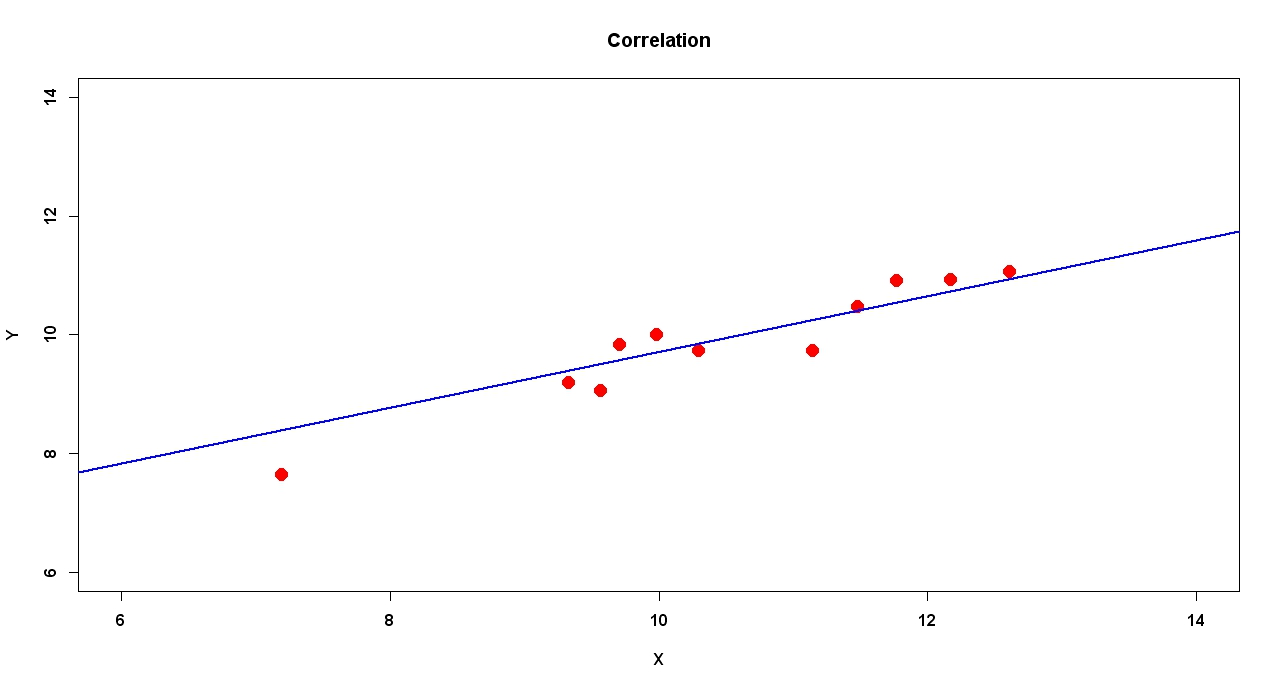
\includegraphics[width=1.05\linewidth]{../IntroStats/CorTest2}
\end{figure}
{

Correlation Coefficient : $r = 0.922$
}


\begin{figure}
\centering
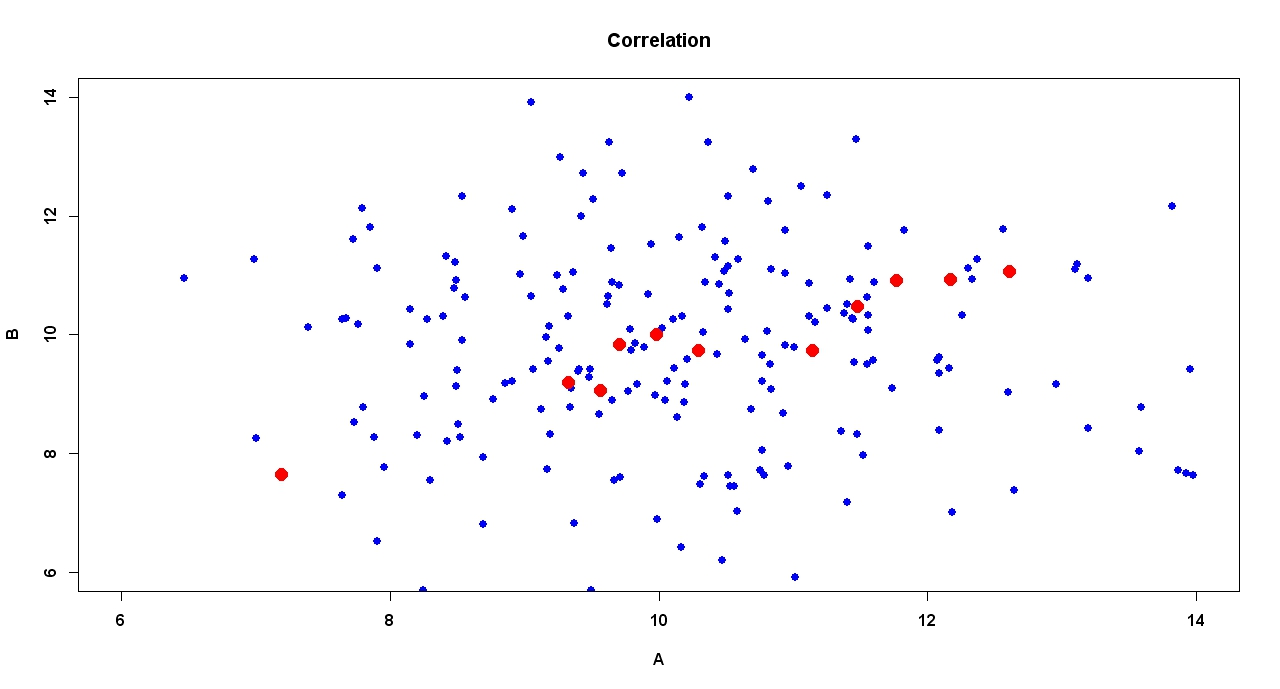
\includegraphics[width=1.05\linewidth]{../IntroStats/CorTest3}
\end{figure}

{

True Correlation Coefficient : $rho \approx 0$
}

%--------------------------------------------------------------------%


\subsection{Significance Test of the Correlation Estimate}
\Large
\vspace{-1cm}
\textbf{Testing using Student's t-distribution}
\vspace{0.5cm}

For pairs from an uncorrelated bivariate normal distribution, the sampling distribution of Pearson's correlation coefficient follows Student's t-distribution with degrees of freedom n - 2. 


%--------------------------------------------------------------------%

\subsection{Significance Test of the Correlation Estimate}
\Large
\vspace{-1cm}
\textbf{Testing using Student's t-distribution}
\vspace{0.5cm}

Specifically, if the underlying variables have a bivariate normal distribution, the variable
\[ t_{TS} = r\sqrt{\frac{n-2}{1 - r^2}} \]


%--------------------------------------------------------------------%

\subsection{Significance Test of the Correlation Estimate}
\Large
\vspace{-1cm}
\textbf{Testing using Student's t-distribution}
\vspace{0.5cm}

Test statistic follows follows Student's t-distribution with degrees of freedom n - 2. Compare the test statistic to quantile with $n-2$ degrees of freedom for specified confidence level.

%--------------------------------------------------------------------%

%--------------------------------------------------------------------%

\subsection{Significance Test of the Correlation Estimate}
\Large
\vspace{-1.0cm}
\textbf{Example}

\begin{itemize}
\item Sample Size : $n = 0.10$
\item Correlation Coefficient : $r = 0.80$
\end{itemize}
\vspace{0.2cm}

\[ t_{TS} \; = \; r\sqrt{\frac{n-2}{1 - r^2}} \; = \; 0.8 \sqrt{\frac{10-2}{1 - 0.64}}  \]
\vspace{0.2cm}
\[ t_{TS} = 0.8 \sqrt{\frac{8}{0.36}} \; = \; 4.21 \]

  


\Large
\begin{center}
\begin{tabular}{|c||c|c|c|c|}
\hline dfs ($\nu$) &  & $0.025$ & $0.05$ &  \\ \hline
\hline $\ldots$ &  & $\ldots$ & $\ldots$ &  \\ 
\hline 9 & $\ldots$ &  & 2.262  &  $\ldots$ \\ 
\hline 10 & $\ldots$ & & 2.228   & $\ldots$ \\ 
\hline 11 & $\ldots$ & & 2.201    & $\ldots$ \\ 
\hline 12 & $\ldots$ & & 2.179   & $\ldots$ \\ 
\hline \phantom{spaces} & \phantom{spaces} & \phantom{spaces}  & \phantom{spaces} & \phantom{spaces} \\ 
\hline 
\end{tabular} 
\end{center}
\begin{itemize}
\item[df] : degrees of freedom
\end{itemize}
\newpage
\subsection*{Test for Significant Correlation}
Getting a correlation coefficient is generally only half the story; you will want to know if the relationship is statistically significant. There is a more complex command called \texttt{\textbf{cor.test()}}. This command additionally provides a hypothesis test for the correlation estimate. The null and alternative hypotheses are as follows.

\begin{itemize}
\item[Ho] : The correlation coefficient for the population of values is zero. \\(i.e. No linear relationship.)
\item[Ha] : The coefficient is not zero. \\ (i.e. Linear relationship exists.)
\end{itemize}
{

\begin{framed}
\begin{verbatim}
> cor.test(X,Y)

Pearson's product-moment correlation

data:  X and Y
t = 2.9107, df = 8, p-value = 0.01957
alternative hypothesis: true correlation is not equal to 0
95 percent confidence interval:
0.1596151 0.9278331
sample estimates:
cor 
0.7171676 


\end{verbatim}
\end{framed}
}

\begin{itemize}
\item A confidence interval for the coefficient is provided for in the \texttt{R} output. 
\item If the interval includes 0 then we fail to reject the null hypothesis.
\end{itemize}


\end{document}
library(MASS)
Z = mvrnorm(12,c(10,10),sigma) 
sigma=matrix(c(2.8,0,0,2.8),nrow=2)

while(cor(Z)[1,2] < 0.7)
 {
 Z = mvrnorm(12,c(10,10),sigma) 
 }

X= round(Z[,1],3)
Y= round(Z[,2],3)
 
while(cor(Z)[1,2] <0.6)
 {
 Z = mvrnorm(360,c(10,10),sigma) 
 }

A= round(Z[,1],3)
B= round(Z[,2],3)

plot(X,Y,pch=16,col="red",cex=1.8,xlim=c(6,14),ylim=c(6,14),font.lab=2,font.axis=2,main="Correlation")

plot(A,B,pch=16,col="blue",cex=1.2,xlim=c(6,14),ylim=c(6,14),font.lab=2,font.axis=2,main="Correlation")
points(X,Y,pch=16,col="red",cex=1.8)

plot(X,Y,pch=16,col="red",cex=1.8,xlim=c(6,14),ylim=c(6,14),font.lab=2,font.axis=2,main="Correlation")
abline(coef(lm(Y~X)),col="blue",lwd=1.5)



%-------------------------------------------------%

\section{Correlation}

This requires a simple calculation based in values given and the relevant formula.

The formula for the Correlation estimate is as follows.

% http://www.statstutor.ac.uk/resources/uploaded/spearmans.pdf

%========================================================================%


\subsubsection*{Implementation}
The relevant \texttt{R} command to compute the correlation coefficient estimate is simply \texttt{\textbf{cor()}}.

%
%\begin{framed}
%\begin{verbatim}
%cor(immer$Y1,immer$Y2)
%
%cor(iris[,1],iris[,3])
%\end{verbatim}
%\end{framed}


%======================================================== %
%\begin{figure}
%\centering
%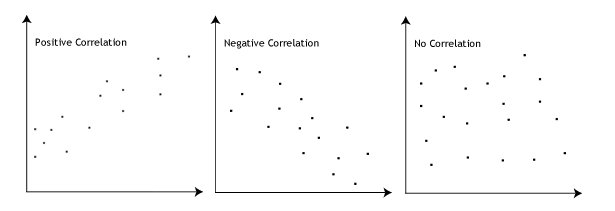
\includegraphics[width=0.7\linewidth]{Regre1}
%\end{figure}


%\begin{figure}[h!]
%\centering
%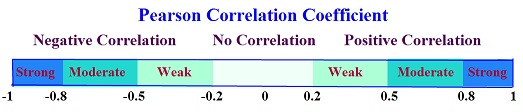
\includegraphics[width=0.9\linewidth]{pearson-correlation-coefficient-interpretation}
%\end{figure}

\subsection*{Test for Significant Correlation}
Getting a correlation coefficient is generally only half the story; you will want to know if the relationship is statistically significant. There is a more complex command called \texttt{\textbf{cor.test()}}. This command additionally provides a hypothesis test for the correlation estimate. The null and alternative hypotheses are as follows.

\begin{itemize}
\item[Ho] : The correlation coefficient for the population of values is zero. \\(i.e. No linear relationship.)
\item[Ha] : The coefficient is not zero. \\ (i.e. Linear relationship exists.)
\end{itemize}
{

\begin{framed}
\begin{verbatim}
> cor.test(X,Y)

Pearson's product-moment correlation

data:  X and Y
t = 2.9107, df = 8, p-value = 0.01957
alternative hypothesis: true correlation is not equal to 0
95 percent confidence interval:
0.1596151 0.9278331
sample estimates:
cor 
0.7171676 


\end{verbatim}
\end{framed}
}

\begin{itemize}
\item A confidence interval for the coefficient is provided for in the \texttt{R} output. 
\item If the interval includes 0 then we fail to reject the null hypothesis.
\end{itemize}



The Pearson correlation coefficient is computed using the
following formula

\begin{multicols}{2}
\begin{itemize}
\item $\sum x$ \item $\sum y$ \item $\sum xy$ \item $\sum x^2$
\item $\sum y^2$
\end{itemize}

\end{multicols}

\begin{center}
\begin{tabular}{|ccc|ccc|ccc|ccc|ccc|}
\hline
& X & & & Y & & &  $X^2$ & & &  $Y^2$ & & &  XY & \\
& 1.0 & & & 10.6 & & &  1.00 & & &  36 & & &  90 & \\ \hline
& 1.2 & & & 12.5 & & &  1.44 & & &  36 & & &  90 & \\ \hline
& 1.6 & & & 14.7 & & &  2.56 & & &  36 & & &  90 & \\ \hline
& 1.7 & & & 16.7 & & &  225 & & &  36 & & &  90 & \\ \hline
& 1.8 & & & 18.7 & & &  225 & & &  36 & & &  90 & \\ \hline
& 2.1 & & & 22.1 & & &  4.41 & & &  36 & & &  90 & \\ \hline


\end{tabular}
\end{center}

\begin{framed}
\[
r = { \; n \sum xy - \sum x \sum y   \; \over \left[\;\sqrt{n \sum (x^2) - (\sum x)^2} \;\right] \times  \left[ \;\sqrt{n \sum (y^2) - (\sum y)^2}\; \right]}
\]
\end{framed}


\subsection*{The Coefficient of Determination}
\begin{itemize}
\item The coefficient of determination $R^2$ is the proportion of variability in a data set that is accounted for by the linear model. 
\item Equivalently $R^2$ provides a measure of how well future outcomes are likely to be predicted by the model.

\item For simple linear regression, it can be computed by squaring the correlation coefficient. It is not specifically defined that way. 
\item This relationship is co-incidental when there are just two variables.
\end{itemize}
\begin{framed}
\begin{verbatim}
> summary(lm(Y~X))

Call:
lm(formula = Y ~ X)
....

Coefficients:
Estimate Std. Error t value  Pr(>|t|)
(Intercept) -18.5506    41.4156  -0.448    0.6661
X             1.1855     0.4073   2.911    0.0196 *

Residual standard error: 3.884 on 8 degrees of freedom
Multiple R-squared:  0.5143,    Adjusted R-squared:  0.4536 
F-statistic: 8.472 on 1 and 8 DF,  p-value: 0.01957

\end{verbatim}
\end{framed}
